\documentclass[a4paper,10pt]{article}\setlength{\textheight}{10in}\setlength{\textwidth}{6.5in}\setlength{\topmargin}{-0.125in}\setlength{\oddsidemargin}{-.2in}\setlength{\evensidemargin}{-.2in}\setlength{\headsep}{0.2in}\setlength{\footskip}{0pt}\usepackage{amsmath}\usepackage{fancyhdr}\usepackage{enumitem}\usepackage{hyperref}\usepackage{xcolor}\usepackage{graphicx}\usepackage[export]{adjustbox}\usepackage{caption}\usepackage{float}\usepackage{booktabs}\pagestyle{fancy}

\lhead{Name: \rule{5cm}{0.5pt}}
\chead{M.Number: \rule{2cm}{0.5pt}}
\rhead{KDDM1 VO (INP.31101UF)}
\fancyfoot{}

\begin{document}
\begin{enumerate}[topsep=0mm, partopsep=0mm, leftmargin=*]





%%% Question 1
{\color{blue}
\item\textit{Visual Data Analysis}. Given the dataset ``task1-dataset.ods'' (available in TeachCenter), which comprises a number of features. Provide a number of meaningful visualisations (4 visualisations) that show key properties of the dataset and dependencies. Based on the visualisations provide your interpretation and insights. 
\begin{enumerate}
	\item What pre-processing did your do? (e.g., Did you create new features? Did you normalise the data? Did you filter the dataset? Extended with another dataset?)
	\item What are the most relevant dependencies between the features (selection of the figures)?
	\item Provide a series of meaningful plots that show a specific relationship (dependency) or characteristic of the dataset
	\item Provide a summary of the main insights
\end{enumerate}
}

%%% Your answer here

\textbf{Answer (a)} - Preprocessing steps:
    \begin{itemize}
        \item First preprocesing step
        \item Second step
        \item ...
    \end{itemize}
    
\textbf{Answer (b)} - List of main dependencies:
    \begin{itemize}
        \item First dependency
        \item ...
    \end{itemize}
    
    
\textbf{Answer (b) and (c)}
% First visualisation
    \begin{figure}[H]
        \centering
        \adjustbox{frame}{
            \includegraphics[width=0.8\textwidth]{example-image}
        }
        \caption{Please provide an explanation for the visualisation - (i) Why this kind of visualisation? (ii) What kind of dependency is being shown? (iii) What are potential interpretations?}
        \label{fig:plot1}
    \end{figure}
    % Second visualisation
    \begin{figure}[H]
        \centering
        \adjustbox{frame}{
            \includegraphics[width=0.8\textwidth]{example-image}
        }
        \caption{Please provide an explanation for the visualisation}
        \label{fig:plot2}
    \end{figure}
    % Third visualisation
    \begin{figure}[H]
        \centering
        \adjustbox{frame}{
            \includegraphics[width=0.8\textwidth]{example-image}
        }
        \caption{Please provide an explanation for the visualisation}
        \label{fig:plot3}
    \end{figure}
    % Fourth visualisation
    \begin{figure}[H]
        \centering
        \adjustbox{frame}{
            \includegraphics[width=0.8\textwidth]{example-image}
        }
        \caption{Please provide an explanation for the visualisation}
        \label{fig:plot4}
    \end{figure}

\textbf{Answer (d)} - Short summary of the main insights (with references to the corresponding image)
    \begin{itemize}
        \item Finding \#1, as illustrated in Figure~\ref{fig:plot1} one ...
        \item ...
    \end{itemize}






\clearpage
{\color{blue}
\newpage\item\textit{Correlation}. Given a dataset, which consists of 1,000 variables (hint: most of them are just random), the goal is to find the relationships between variables, i.e., which and how do the variables relate to each other; what are the dependencies.
The dataset ``task2-dataset.csv'' can be downloaded from TeachCenter.
\begin{enumerate}
	\item Which methods did you apply to find the relationships, and why?
	\item Which relationships did you find and how do you characterise the relationships (e.g., variable ``Lurkowl (Strix umbra \#1068)'' to ``Frosthawk (Accipiter glacies \#1064)'' is linear with correlation found via method X of 0.9)?
	\item Which causal relationships between the variables can you find (e.g., variable ``Rattlepuff (Lynx rattleus \#1067)'' causes ``Slingshark (Carcharodon slingus \#1068)'')?
\end{enumerate}
}

%%% Your answer here
\textbf{Answer (a)} - Method and motivation:
    \begin{enumerate}
        \item First Method - Why chosen (one sentence)
        \item Second Method
        \item ...
    \end{enumerate}

\textbf{Answer (b)}
    \begin{center}
    \begin{tabular}{lllll}
    \toprule
    \textbf{Variable 1} & \textbf{Variable 2} & \textbf{Type of dependency} & \textbf{Method} & \textbf{Value} \\ \midrule
    × & × & × & × & × \\
    × & × & × & × & × \\
    \bottomrule
    \end{tabular}
    \end{center}

\textbf{Answer (c)}




{\color{blue}
\clearpage\item \textit{Outliers/Anomalies}. Given two types of anomalies: (1) anomalies are defined to be \textbf{datapoints} in low density regions, (2) anomalies are \textbf{regions} of low density.
\begin{enumerate}
\item For both anomalies please create/draw a dataset of 2 features (x and y axis), with 3 anomalies and many normal data points (the normal datapoints should be marked, e.g., green colour)
\item Name the algorithms or describe the algorithmic way of how to identify this anomalous behaviour (you may also describe any necessary preprocessing)
\item Name the assumptions made by your algorithms
\end{enumerate}}




\textbf{Answer (a)} - Draw two datasets % Update the images to reflect a scatterplot of a dataset
    \begin{center}
    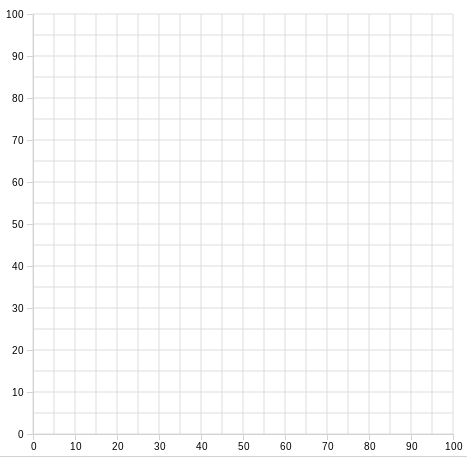
\includegraphics[width=.4\textwidth]{empty-dataset-1.png}
        \hspace{2cm}
    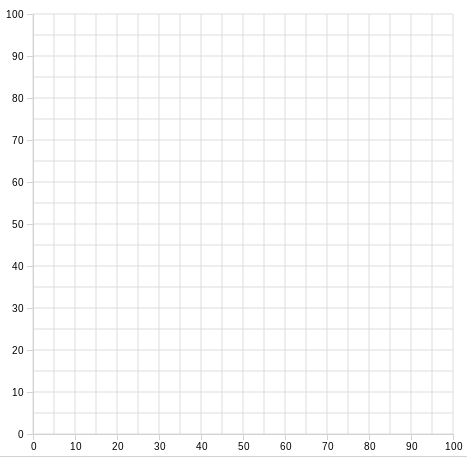
\includegraphics[width=.4\textwidth]{empty-dataset-2.png}
    \end{center}


\textbf{Answer (b)} - Describe the algorithms 
\begin{description}
	\item[Dataset 1] ``Name of algorithm/method'' followed by a justification, why the method has been selected...
	\item[Dataset 2] ...
\end{description}


\textbf{Answer (c)} - Describe the main assumptions \\
\begin{center}
\begin{tabular}{ll}
\toprule
\textbf{Algorithm} & \textbf{Assumption} \\ \midrule
× & × \\
× & × \\ 
\bottomrule
\end{tabular}
\end{center}


%%% Your answer here



{\color{blue}
\clearpage\item\textit{Missing Values}. The dataset ``task4-dataset.csv'' (available on TeachCenter) contains a number of missing values. Try to reconstruct why the missing values are missing? What could be an explanation?
\begin{enumerate}
	\item What are the dependencies in the dataset?
	\item What could be reasons for the missingness?
	\item What strategies are applicable for the features to deal with the missing values?
	\item For each feature provide an estimate of the arithmetic mean (before and after applying the strategies to deal with missing values)?
\end{enumerate}
}

%%% Your answer here
\textbf{Answer (a)} - Describe the dependencies in the dataset
\begin{center}
\begin{tabular}{lll}
\toprule
\textbf{X} & \textbf{Y} & \textbf{Type of dependency} \\ \midrule
× & × & × \\
× & × & × \\
\bottomrule
\end{tabular}
\end{center}

\textbf{Answer (b)} - Describe the reason for missingness
\begin{center}
\begin{tabular}{ll}
\toprule
\textbf{Variable} & \textbf{Reason} \\ \midrule
× & × \\
× & × \\
\bottomrule
\end{tabular}
\end{center}

\textbf{Answer (c)} - Describe the strategies for dealing with missing values
\begin{center}
\begin{tabular}{ll}
\toprule
\textbf{Variable} & \textbf{Strategy} \\ \midrule
× & × \\
× & × \\
\bottomrule
\end{tabular}
\end{center}

\textbf{Answer (d)} - Arithmetic mean of original dataset (with the missing values), and the one after applying the strategies
\begin{center}
\begin{tabular}{lll}
\toprule
\textbf{Variable} & \textbf{Before Strategy} & \textbf{After Strategy} \\ \midrule
× & × & × \\
× & × & × \\
\bottomrule
\end{tabular}
\end{center}

\end{enumerate}
\end{document}
